\documentclass[11pt, letterpaper]{article}
\usepackage[margin=0.5in]{geometry}
\usepackage{graphicx}
\usepackage{float}
\usepackage{placeins}

\begin{document}

\title{MicroDNA}
\author{Mathis Fituwi}
\maketitle

\section{Introduction}

MicroDNA is a subtype of Extrachromosomal Circular DNA, as it is a small (roughly a few hundred base pairs) circular piece of DNA that exists outside chromosomes and is derived from genomic DNA. In this project, we want to reliably identify suspected microDNA circles based on alignment data from BAM files generated by sequencing and to create a confidence metric to distinguish potentially true circular DNA from false signals. In our case, we are using a BAM file from the 1000 Genomes Project (NA12878, chromosome 20, low-coverage Illumina sequencing aligned with Burrows-Wheeler Aligner).
\vspace{\baselineskip}

From here, we take reads from our BAM file and apply CIGAR operations to identify potential tags based on soft-clipping either ends of the read as these regions could indicate a circular DNA link. These tags then get grouped into regions and analyzed to see if we can find any strong evidence of a read being a circular DNA. With a support and score metric, we pick out our most likely candidates and return then as predicted circles with it's respective confidence score.

\vspace{\baselineskip}

Our findings show that potential microDNA locations are distributed across the genome, with some regions displaying notably high confidence suggesting they may represent true microDNA.


% \vspace{\baselineskip}

% test

% \vspace{\baselineskip}

% test

% \vspace{\baselineskip}

% test


    
    

\subsection{Results}

\begin{figure} [H]
    \centering
    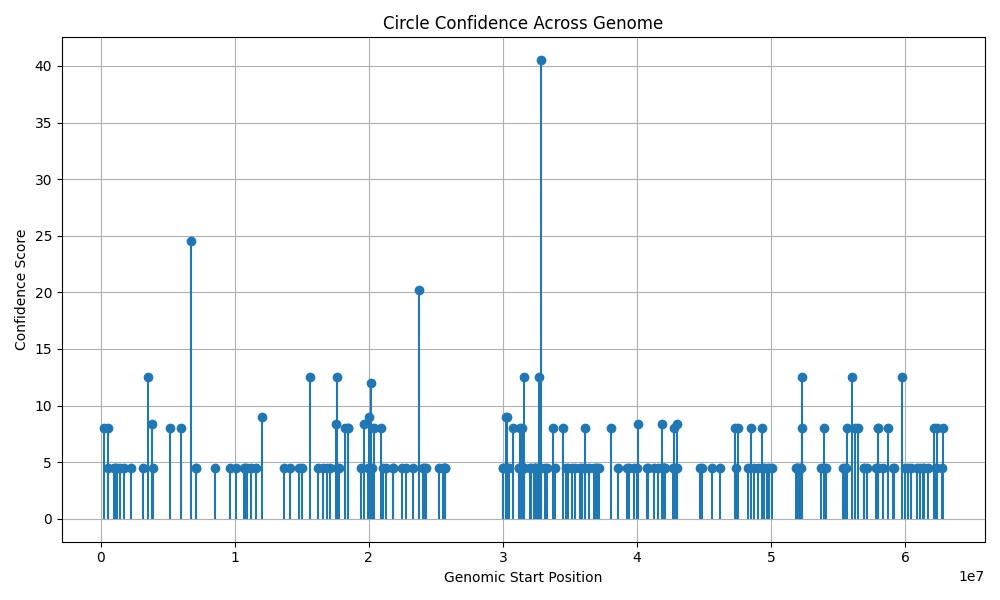
\includegraphics[width=0.7\linewidth]{circle_confidence.png}
    \caption{Confidence distribution of reads from \textit{NA12878} chromosome 20 BAM file.}
    \label{fig:circle-confidence}
\end{figure}

In Figure 1, we see that the confidence distribution plot shows predicted microDNA circles along chromosome 20, with their genomic starting positions on the x-axis and confidence scores on the y-axis. Across the board, regions display moderate confidence values, with a few peaks standing out significantly. These abnormally high-confidence regions may definitely reflect potential locations of circularization.


\subsection{Method}


To detect potential microDNA circles, we begin by scanning soft-clipped reads from a BAM file. Soft clipping in the CIGAR string marks where parts of the read didn’t perfectly align, but these regions may still reveal points of a circular junction. We collect those positions and label them as tags, also noting whether they come from the left or right side of the read.

\vspace{\baselineskip}

Then we group those tags into bins of a fixed size. This windowing helps narrow down regions where soft-clipped tags are clustering. For each bin, if both left and right tags are present, we calculate its support by counting how many tags are in that bin. The more tags, the stronger the evidence for a possible circle.

\vspace{\baselineskip}

From there, we take the median position of the left tags and the median of the right tags to define a rough start and end point. We then calculate a \textbf{score}, which is the support divided by the distance between those points:

\[
\text{score} = \frac{\text{support}}{\text{span} + 1}
\]

This keeps circles tight, and if tags are too spread out, the score falls.

\vspace{\baselineskip}


Finally, we define a confidence metric as just support times score:

\[
\text{confidence} = \text{support} \times \text{score}
\]

This balances how many reads back up a circle and how close they are. If both the score and support are high enough, we keep it as a predicted microDNA circle.


\subsection{Reproducibility}
To replicate these experiments, follow these steps:

\begin{verbatim}
$ git clone git@github.com:MatFit/ProjectDNA.git
$ cd ProjectDNA
$ python3 src/cli.py \
        data/sample.bam \
        -o visuals/test_circles.csv \
        --min-score 1.5 \ 
$ python3.10 src/visuals.py \
        csvs/test_circles.csv \


\end{verbatim}
\textit{cli.py} is used as a simple interface to make the process of using different BAM files more modular. \textit{visual.py} is used to display the distribution of circle confidence using a stem plot for user viewership.

\vspace{\baselineskip}


\textbf{NOTE}: This repository only contains a subset of the original \textit{NA12878} chromosome 20 BAM file, as the full file is too large to be kept in the public repository.




\end{document}
